%%%%%%%% CSCI 467 EXAMPLE LATEX SUBMISSION FILE %%%%%%%%%%%%%%%%%
%%%%%%%% Adapted from the ICML 2021 EXAMPLE LATEX SUBMISSION FILE %%%%%%%%%%%%%%%%%

\documentclass{article}

% Recommended, but optional, packages for figures and better typesetting:
\usepackage[utf8]{inputenc}
\usepackage{microtype}
\usepackage{graphicx}
\usepackage{subfigure}
\usepackage{booktabs} % for professional tables

% hyperref makes hyperlinks in the resulting PDF.
% If your build breaks (sometimes temporarily if a hyperlink spans a page)
% please comment out the following usepackage line and replace
% \usepackage{icml2021} with \usepackage[nohyperref]{icml2021} above.
\usepackage{hyperref}

% Attempt to make hyperref and algorithmic work together better:
\newcommand{\theHalgorithm}{\arabic{algorithm}}

% Use the following line for the initial blind version submitted for review:
%\usepackage{icml2021}

% If accepted, instead use the following line for the camera-ready submission:
\usepackage[accepted]{icml2021}

\begin{document}

\twocolumn[
\icmltitle{Housing Price Prediction}

\begin{icmlauthorlist}
\icmlauthor{Author One}{}
\icmlauthor{Author Two}{}
\icmlauthor{Author Three}{}
\end{icmlauthorlist}

\vskip 0.3in
]

% this must go after the closing bracket ] following \twocolumn[ ...

% This command actually creates the footnote in the first column
% listing the affiliations and the copyright notice.
% The command takes one argument, which is text to display at the start of the footnote.
% The \icmlEqualContribution command is standard text for equal contribution.
% Remove it (just {}) if you do not need this facility.

%\printAffiliationsAndNotice{}  % leave blank if no need to mention equal contribution
%\printAffiliationsAndNotice{\icmlEqualContribution} % otherwise use the standard text.

\begin{abstract}

This project investigates house price prediction using the Kaggle House Prices dataset, with a focus on comparing linear, nonlinear, and ensemble-based machine learning models. We evaluated Linear Regression, Ridge, Lasso, Gradient Boosting, and XGBoost, together with hybrid and stacking approaches. Our preprocessing pipeline included missing value handling, categorical feature encoding, and feature transformation. We found that purely linear models were insufficient for capturing complex relationships in housing data, while nonlinear ensemble methods significantly improved prediction performance. Furthermore, combining linear and nonlinear models through hybrid averaging and stacking produced more stable and accurate predictions than individual models. Our results highlight the importance of feature engineering and ensemble learning in structured regression tasks.

\end{abstract}

\section{Introduction}

This project investigates house price prediction using the Kaggle House Prices: Advanced Regression Techniques dataset \href{https://www.kaggle.com/competitions/house-prices-advanced-regression-techniques}
{Kaggle House Prices Competition}. The task involves predicting housing sale prices from a mixture of numerical and categorical housing features, including property size, quality, neighborhood information, and construction details. Because housing prices depend on complex feature interactions and nonlinear relationships, this dataset provides an interesting setting for studying the performance and limitations of different machine learning models.

Our project began as a comparison of regression approaches including Linear Regression, Ridge, Lasso, and nonlinear boosting methods. Over time, the project evolved into a more analytical investigation of when linear models become insufficient and whether combining linear and nonlinear models can improve the prediction's performance.We explored ensemble approaches including weighted hybrid models and stacking architectures.

When reviewing prior work and public Kaggle submissions for this competition, we found that top-performing solutions relied heavily on feature engineering and ensemble learning techniques. The solution by \href{https://www.kaggle.com/code/jesucristo/1-house-prices-solution-top-1}
{House Prices Solution [top 1]} \cite{top1_kaggle} demonstrated the effectiveness of combining multiple regression and boosting models for improved  performance. We also found \href{https://www.kaggle.com/code/mviola/house-prices-eda-lasso-lightgbm-0-11635}
{House Prices EDA, Lasso, LightGBM} \cite{lasso_lgbm} particularly useful for combining linear regularized models such as Lasso with nonlinear boosting approaches such as LightGBM. These prior solutions helped with our feature engineering process.

Inspired by these approaches, we investigate whether combining linear and nonlinear models can consistently outperform individual models alone. Our work focuses on predictive accuracy, and the effectiveness of ensemble learning in structured regression tasks.



\begin{figure*}[t]
    \centering
    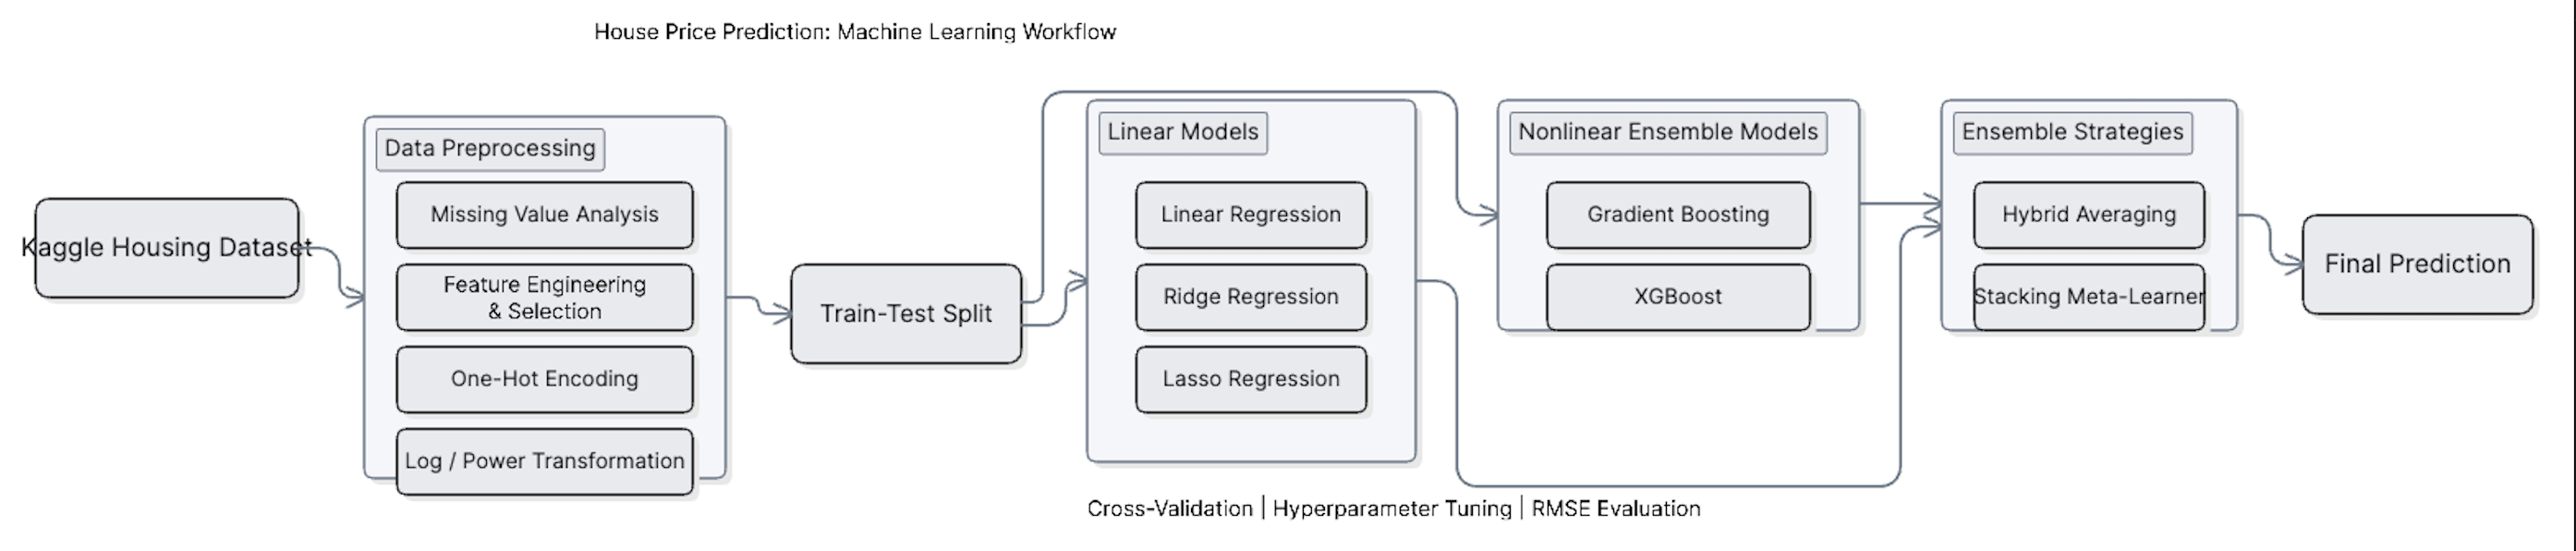
\includegraphics[width=\textwidth]{pipeline_2.png}
    \caption{Overview of the machine learning workflow used for house price prediction.}
    \label{fig:pipeline}
\end{figure*}

\section{Methods}

Figure~\ref{fig:pipeline} presents the overall machine learning workflow used in this project. Our methodology consists of four main stages: data preprocessing, linear regression baselines, nonlinear ensemble models, and ensemble combination strategies.

\subsection{Data Preprocessing}

The Kaggle House Prices dataset contains both numerical and categorical features with substantial missing values. Missing categorical values representing the absence of a property feature (e.g., pool or fence) were encoded accordingly, while numerical missing values were imputed using the median. Categorical variables were transformed using one-hot encoding.

To improve model stability and reduce skewness, logarithmic and power transformations were applied to selected variables. In particular, the target variable \texttt{SalePrice} exhibited a strongly right-skewed distribution, motivating the use of a logarithmic transformation to reduce the influence of outliers and improve distribution symmetry.

\subsection{Linear Regression Models}

We first established baseline performance using ordinary least squares linear regression. These models served as  baselines for analyzing the limitations of linear assumptions in housing price prediction.
To improve generalization and reduce overfitting, we additionally evaluated Ridge and Lasso regression models. Ridge regression introduces an L2 regularization penalty, while Lasso regression applies an L1 penalty that performs implicit feature selection. Regularization strengths were selected using cross-validation to balance model complexity and performance.

\subsection{Nonlinear Ensemble Models}

To capture nonlinear relationships and complex feature interactions within the housing dataset, we further evaluated nonlinear ensemble methods including Gradient Boosting Regression and XGBoost. Unlike linear models, boosting methods iteratively train decision trees on residual errors from previous predictors, enabling the models to learn nonlinear structures in the data.

 We additionally conducted hyperparameter sensitivity analysis using cross-validation together with grid search and randomized search procedures. Hyperparameters including learning rate, tree depth, number of estimators, subsampling ratio, and minimum leaf size were tuned to improve predictive performance and reduce overfitting.

\subsection{Ensemble Combination Strategies}

To systematically study whether combining linear and nonlinear models improves prediction performance, we implemented both weighted hybrid averaging and stacking architectures.

Our weighted hybrid model combines predictions from Ridge regression and Gradient Boosting through a convex combination:
\[
\hat y_{hybrid}= \alpha \hat y_{ridge} + (1-\alpha)\hat y_{GB}
\]
where $\alpha \in [0,1]$ controls the relative contribution of the linear Ridge regression model and the nonlinear Gradient Boosting model.

We further implemented stacking architectures in which predictions from multiple base learners were used as inputs to a meta-learner that generated the final prediction. Multiple ensemble configurations were evaluated, including combinations of regularized linear models and nonlinear boosting models. These ensemble approaches aim to leverage the strengths of different model families while reducing the weaknesses of individual predictors.


\section{Figures}

You may want to include figures in the paper to illustrate
your approach and results. Such artwork should be centered,
legible, and separated from the text. Lines should be dark and at
least 0.5~points thick for purposes of reproduction, and text should
not appear on a gray background.

Label all distinct components of each figure. If the figure takes the
form of a graph, then give a name for each axis and include a legend
that briefly describes each curve. Do not include a title inside the
figure; instead, the caption should serve this function.

Number figures sequentially, placing the figure number and caption
\emph{after} the graphics, with at least 0.1~inches of space before
the caption and 0.1~inches after it, as in
Figure~\ref{icml-historical}. The figure caption should be set in
9~point type and centered unless it runs two or more lines, in which
case it should be flush left. You may float figures to the top or
bottom of a column, and you may set wide figures across both columns
(use the environment \texttt{figure*} in \LaTeX). Always place
two-column figures at the top or bottom of the page.

\section{Algorithms}

If you are using \LaTeX, please use the ``algorithm'' and ``algorithmic''
environments to format pseudocode. These require
the corresponding stylefiles, algorithm.sty and
algorithmic.sty, which are supplied with this package.
Algorithm~\ref{alg:example} shows an example.





Tables contain textual material, whereas figures contain graphical material.
Specify the contents of each row and column in the table's topmost
row. Again, you may float tables to a column's top or bottom, and set
wide tables across both columns. Place two-column tables at the
top or bottom of the page.

\section{Citations and References}

Please use APA reference format regardless of your formatter
or word processor. If you rely on the \LaTeX\/ bibliographic
facility, use \texttt{natbib.sty} and \texttt{icml2021.bst}
included in the style-file package to obtain this format.

Citations within the text should include the authors' last names and
year. If the authors' names are included in the sentence, place only
the year in parentheses, for example when referencing Arthur Samuel's
pioneering work \yrcite{Samuel59}. Otherwise place the entire
reference in parentheses with the authors and year separated by a
comma \cite{Samuel59}. List multiple references separated by
semicolons \cite{kearns89,Samuel59,mitchell80}. Use the `et~al.'
construct only for citations with three or more authors or after
listing all authors to a publication in an earlier reference \cite{MachineLearningI}.


\section{Final instructions}

Do not change any aspects of the formatting parameters in the style files.  In
particular, do not modify the width or length of the rectangle the text should
fit into, and do not change font sizes (except perhaps in the
\textbf{References} section; see below). Please note that pages should be
numbered.


\subsection{Preparing PDF files}

You can download a PDF version of your report to submit to Gradescope with the download PDF icon above the PDF preview in Overleaf.


\bibliography{main}
\bibliographystyle{icml2021}


%%%%%%%%%%%%%%%%%%%%%%%%%%%%%%%%%%%%%%%%%%%%%%%%%%%%%%%%%%%%%%%%%%%%%%%%%%%%%%%
%%%%%%%%%%%%%%%%%%%%%%%%%%%%%%%%%%%%%%%%%%%%%%%%%%%%%%%%%%%%%%%%%%%%%%%%%%%%%%%
% DELETE THIS PART. DO NOT PLACE CONTENT AFTER THE REFERENCES!
%%%%%%%%%%%%%%%%%%%%%%%%%%%%%%%%%%%%%%%%%%%%%%%%%%%%%%%%%%%%%%%%%%%%%%%%%%%%%%%
%%%%%%%%%%%%%%%%%%%%%%%%%%%%%%%%%%%%%%%%%%%%%%%%%%%%%%%%%%%%%%%%%%%%%%%%%%%%%%%
%\appendix
%\section{Appendix}
%If you have any additional results or details you want to report that do not fit within the page limit, you may include them in an appendix here.

%%%%%%%%%%%%%%%%%%%%%%%%%%%%%%%%%%%%%%%%%%%%%%%%%%%%%%%%%%%%%%%%%%%%%%%%%%%%%%%
%%%%%%%%%%%%%%%%%%%%%%%%%%%%%%%%%%%%%%%%%%%%%%%%%%%%%%%%%%%%%%%%%%%%%%%%%%%%%%%


\end{document}


% This document was modified from the file originally made available by
% Pat Langley and Andrea Danyluk for ICML-2K. This version was created
% by Iain Murray in 2018, and modified by Alexandre Bouchard in
% 2019 and 2021. Previous contributors include Dan Roy, Lise Getoor and Tobias
% Scheffer, which was slightly modified from the 2010 version by
% Thorsten Joachims & Johannes Fuernkranz, slightly modified from the
% 2009 version by Kiri Wagstaff and Sam Roweis's 2008 version, which is
% slightly modified from Prasad Tadepalli's 2007 version which is a
% lightly changed version of the previous year's version by Andrew
% Moore, which was in turn edited from those of Kristian Kersting and
% Codrina Lauth. Alex Smola contributed to the algorithmic style files.
